%!TeX root = ../../ccc_main.tex
%!TeX spellcheck = en_GB

\subsection{Goldreich-Goldwasser-Micali from PRG}
Although apparently stronger, the existence of PRF is equivalent to that of Pseudo Random Generators (PRG) with \textit{good} stretch. 
PRFs trivially yields PRGs.
\cite{FOCS:GolGolMic84} instead proposed a tree-like construction of PRFs from PRGs with an expansion factor of $2$\footnote{This is actually implied by PRGs with an expansion factor $1 + p(\secp)^{-1}$ for a given polynomial $p$ through standard amplification techniques.}.
More precisely, let $G : \{0,1\}^\secp \to \{0,1\}^{2\secp}$ be a PRG.
The idea is to sample an initial PRG seed $s$, which serves as PRF key, and define a tree from consecutive application of $G$ where the left child are first $\secp$ bits of $G$'s output, while the right child are last $\secp$ bits.
This is illustrated for height $2$ in Figure~\ref{fig:GGM84:tree_based_prf}.
To evaluate the PRF on input a bit string $(b_1, \ldots, b_n)$, the leaf corresponding to the path identified by those bits (where $0$ means \textit{left-child} and $1$ means \textit{right-child}) is returned.

\begin{figure}[htb]
	\centering
	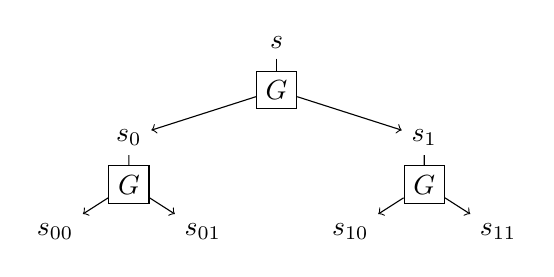
\begin{tikzpicture}[xscale=1.25, yscale=-.6]
		\node (s) at (0,0) {$s$};
		
		\node[draw] (gs) at (0,1) {$G$};
		
		\node (s0) at (-1.5, 2) {$s_0$};
		\node (s1) at (1.5, 2) {$s_1$};
		
		\node[draw] (gs0) at (-1.5, 3) {$G$};
		\node[draw] (gs1) at (1.5, 3) {$G$};
		
		\node (s00) at (-2.25, 4) {$s_{00}$};
		\node (s01) at (-0.75, 4) {$s_{01}$};
		\node (s10) at (0.75, 4) {$s_{10}$};
		\node (s11) at (2.25, 4) {$s_{11}$};
		
		%========================================================================
		% Arrows
		\draw[-] (s) to (gs);
		\draw[-] (s0) to (gs0);
		\draw[-] (s1) to (gs1);
		\draw[->] (gs) to (s0);
		\draw[->] (gs) to (s1);
		\draw[->] (gs0) to (s00);
		\draw[->] (gs0) to (s01);
		\draw[->] (gs1) to (s10);
		\draw[->] (gs1) to (s11);
	\end{tikzpicture}
	\caption{\cite{FOCS:GolGolMic84} PRF construction from a PRG $G: \{0,1\}^\secp \to \{0,1\}^{2\secp}$. In the figure, $s$ is the PRF key and $\{0,1\}^2$ is the PRF domain.}
	\label{fig:GGM84:tree_based_prf}
\end{figure}

\begin{figure}[htb]
\centering
\begin{pcarray}{ll}
	\algorithm{
		$\cd{Gen}(1^\secp):$
		}
		{
			Sample a PRG seed $s$
				\\
			\textbf{Return} $s$
		}
		&
	\algorithm{
		$\cd{Eval}(s; x):$
		}
		{
			Parse $x = (b_1, \ldots, b_n) \in \{0,1\}^n$
				\\
			\textbf{Return} $G_{b_n} \circ G_{b_{n-1}} \circ \ldots \circ G_{b_1}(s)$
		}
\end{pcarray}
\caption{PRF from a PRG $G: \{0,1\}^\secp \to \{0,1\}^{2\secp}$. $G_0$ and $G_1$ on input $s$ returns respectively the first and last $\secp$ bits of $G(s)$.}
\label{prot:GGM84:prf_from_prg}
\end{figure}

\begin{theorem}
	\label{theo:GGM84}
	If $G : \{0,1\}^\secp \to \{0,1\}^{2\secp}$ is a secure pseudo-random generator, then $(\cd{Gen}, \cd{Eval})$ described in Figure~\ref{prot:GGM84:prf_from_prg} is a secure PRF.
\end{theorem}
\begin{proof}
	The high level idea is to have $n+1$ hybrids replacing the intermediate values with (lazily maintained) truly random values.
	Formally, in the hybrid $\cd{H}_\ell$ for $\ell \in \{0, \ldots, n\}$, a random function $R: \{0,1\}^\ell \to \{0,1\}^\ell$ is lazily maintained, meaning that its output is sampled only once for its first invocation and stored for future calls.
	Then, on input $(b_1, \ldots, b_n)$, the challenger returns
	\[
		G_{b_n} \circ G_{b_{n-1}} \circ \ldots \circ G_{b_{\ell + 1}} ( H(b_1, \ldots, b_\ell) ).
	\]
	To show $\cd{H}_\ell$ to be indistinguishable from $\cd{H}_{\ell + 1}$, we rely on the PRG's security.
	
	Indeed, given $\mathcal{A}$ distinguishing $\cd{H}_\ell$ from $\cd{H}_{\ell + 1}$ which makes at most $q$ queries, we build $\mathcal{B}$ distinguishing the two distributions
	\[
		\left(G(s_1), \ldots, G(s_q)\right),
			\quad
		\left(u_1, \ldots, u_q\right)
			\quad : \quad
		s_i \sim U(\{0,1\}^\secp)
			, \;
		u_i \sim U(\{0,1\}^{2\secp})
	\]
	and $s_i$, $u_i$ are all mutually independent.
	Note this reduces to the PRG's security up to a factor-$q$ loss through a standard sequence of hybrids.
	\begin{figure}[htb]
	\centering
	\algorithm{$\mathcal{B}^{\mathcal{O}}(u_1, \ldots, u_q):$}{
		Initialize an empty table $H : \{0,1\}^{\ell+1} \to \{0,1\}^{\secp}$ and set a counter $i \gets 1$
			\\
		Run $\mathcal{A}(1^\secp)$ and when it queries the PRF value on $(b_1, \ldots, b_n)$:
			\\
		\t If $H(b_1, \ldots, b_{\ell + 1}) = \perp$: 
			\\
		\t\t Set $\rho_0 || \rho_1 \gets u_i$, increase $i \gets i + 1$
			\\
		\t\t Program $H(b_1, \ldots, b_\ell, 0) \gets \rho_0$ and $H(b_1, \ldots, b_\ell, 1) \gets \rho_1$
			\\
		\t Set $r \gets H(b_1, \ldots, b_{\ell + 1})$
			\\
		\t Reply to $\mathcal{A}$ with $G_{b_n} \circ \ldots \circ G_{b_{\ell + 2}}(r)$
			\\
		When $\mathcal{A}$ output a bit: Return the same bit
	}
	\label{prot:GGM84:prg_loose_reduction}
	\caption{$\mathcal{B}$ reducing a distinguisher for $\cd{H}_{\ell}$ and $\cd{H}_{\ell + 1}$ to $q$ PRG instances.}
	\end{figure}
	
	If $u_1, \ldots, u_q$ are generated with a PRG, $\mathcal{B}$ simulates $\cd{H}_\ell$ perfectly. Conversely if $u_1, \ldots, u_q$ are random it simulates $\cd{H}_{\ell + 1}$.
	Therefore $\adv{\mathcal{A}} = \adv{\mathcal{B}}$.
	As $\cd{H}_0$ and $\cd{H}_\ell$ are the real and ideal games in the pseudorandomness definition, the thesis is proven.
\end{proof}